\chapter{Current State of AMCS}
\label{chapter:stateoftheart}
AMCS provides front end applications for iOS, Android and web that enable access to a variety of features that benefit both lecturers and the audience.
As already established in the introduction, AMCS is a research prototype used to implement and test new components in the ARS context. Most of the features currently in place were designed and developed by different people over the years and therefore all differ variously in terms of UI design and layout.
To keep the scope of this work manageable, this work will mostly focus on all features that audience members will come in contact with when using AMCS.
This section elaborates on the current state of the system by identifying and analyzing all views that allow for access to the different functionalities of AMCS from a student's point of view. 

\section{Web Technologies}
The AMCS front end web page is written using Angular\footnote{https://angular.io (\emph{last access: 01.11.2019})}, a typescript-based front end framework for building mobile and desktop web applications.

\section{Landing Page and Login}
\label{section:landingpage}
When accessing the website\footnote{https://amcs.website (\emph{last access: 01.11.2019})}, students will be shown the landing page of AMCS (see \Cref{fig:landingpage}). A big login button is displayed that will reveal a login form (see \Cref{fig:loginform}) when pressed.
In order to use the system, students have to create an account by providing credentials.
\newline
\newline
Additionally, a subscription to courses is mandatory in order to reasonably use the service. Each course is identified by a PIN code. By typing in the optional PIN code, students will subscribe automatically to the corresponding course. From thereon, students have access to the system. 
 
\begin{figure}
	\centering
	\begin{minipage}[t]{.5\textwidth}
		\centering
 		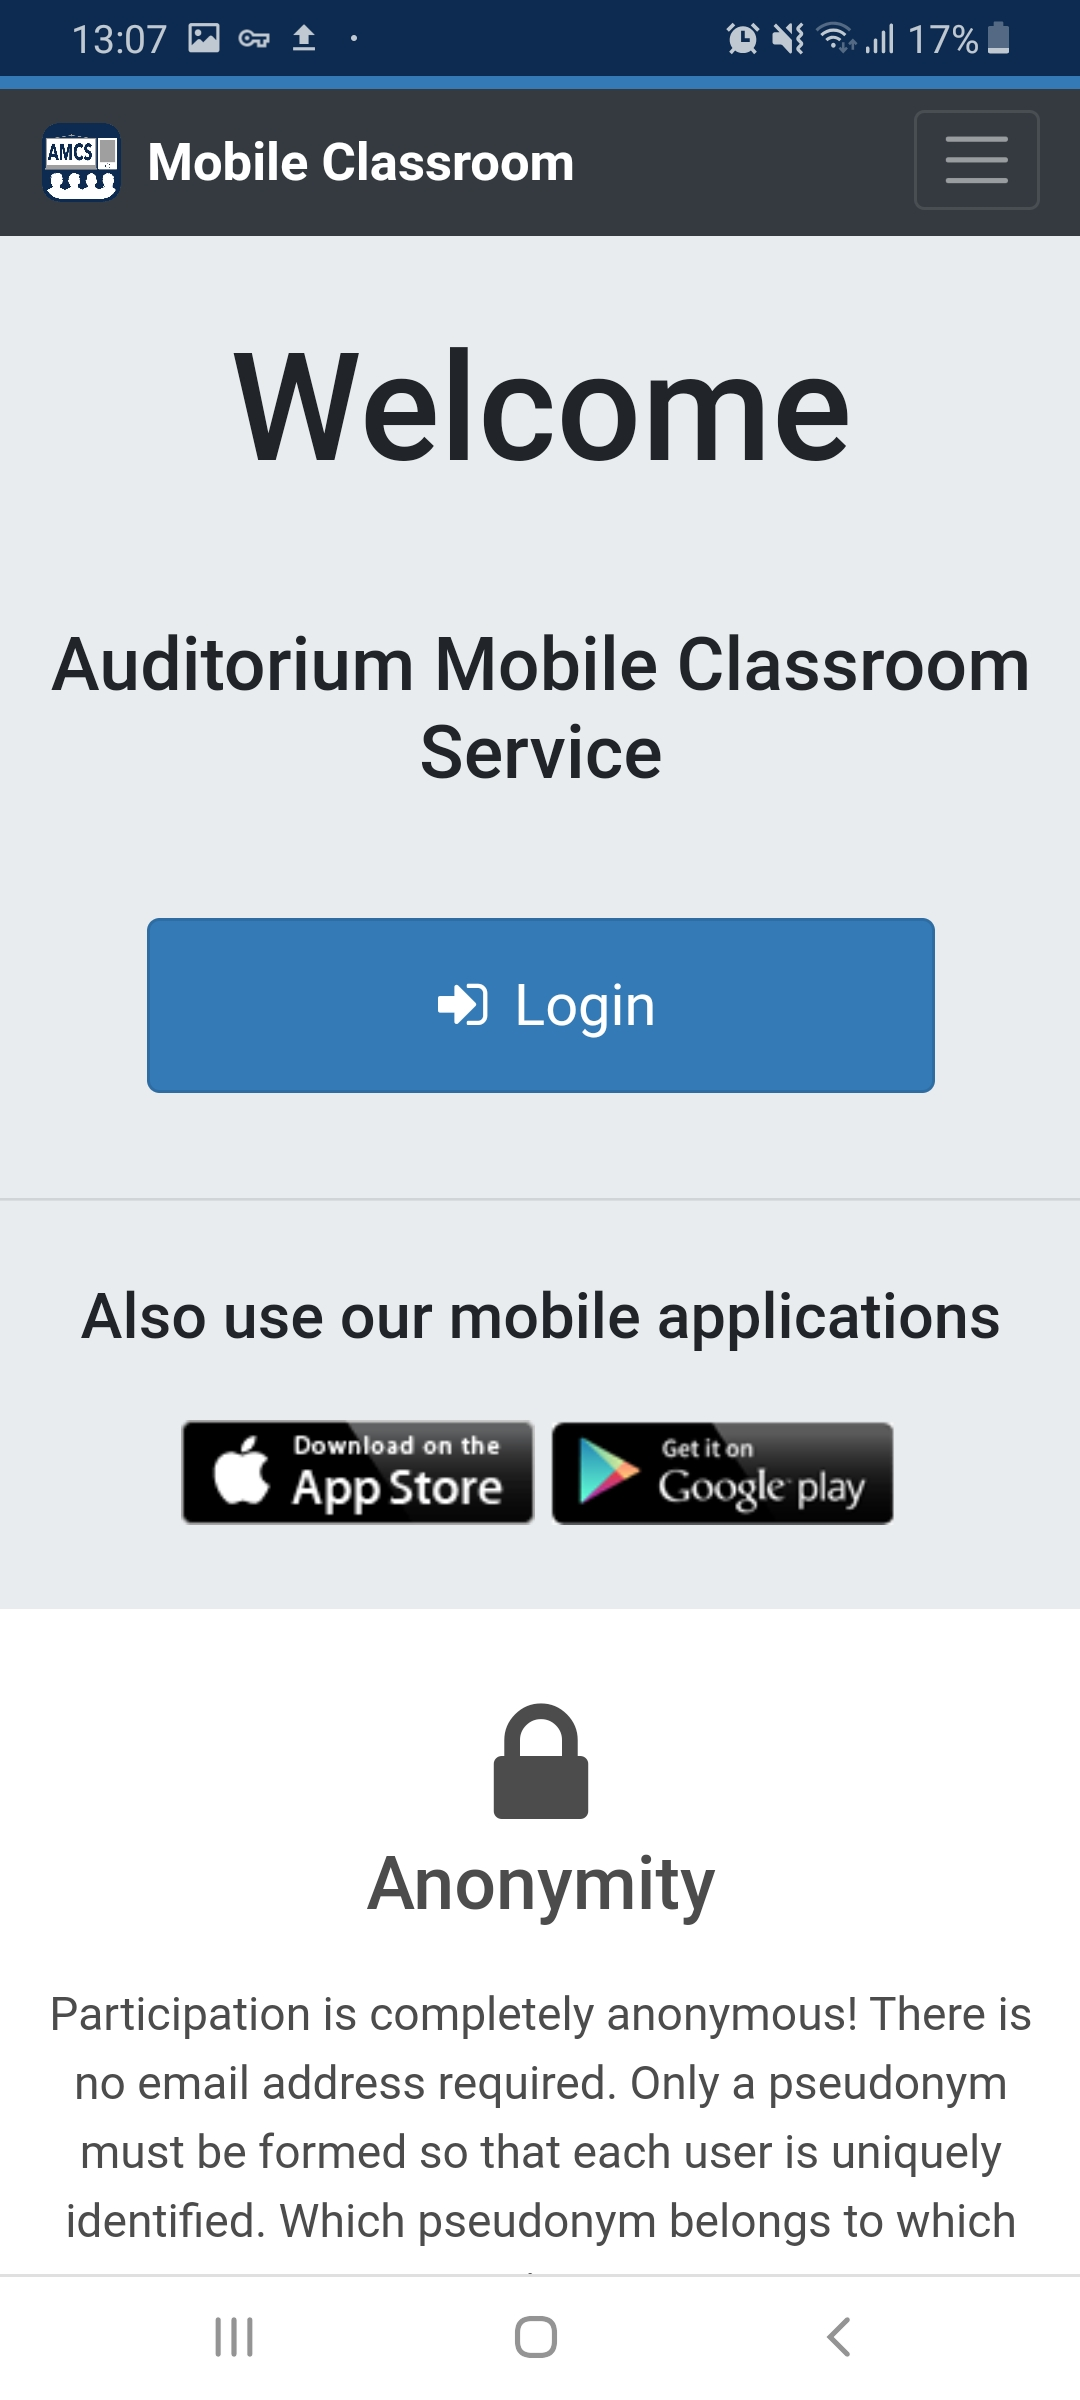
\includegraphics[width=0.95\linewidth]{screenshots/landing_page.jpg}
		\captionsetup{width=.8\linewidth}
		\caption{The landing page of AMCS. This is the initial screen shown when accessing \emph{https://amcs.website}}
		\label{fig:landingpage}
	\end{minipage}%
	\begin{minipage}[t]{.5\textwidth}
		\centering
		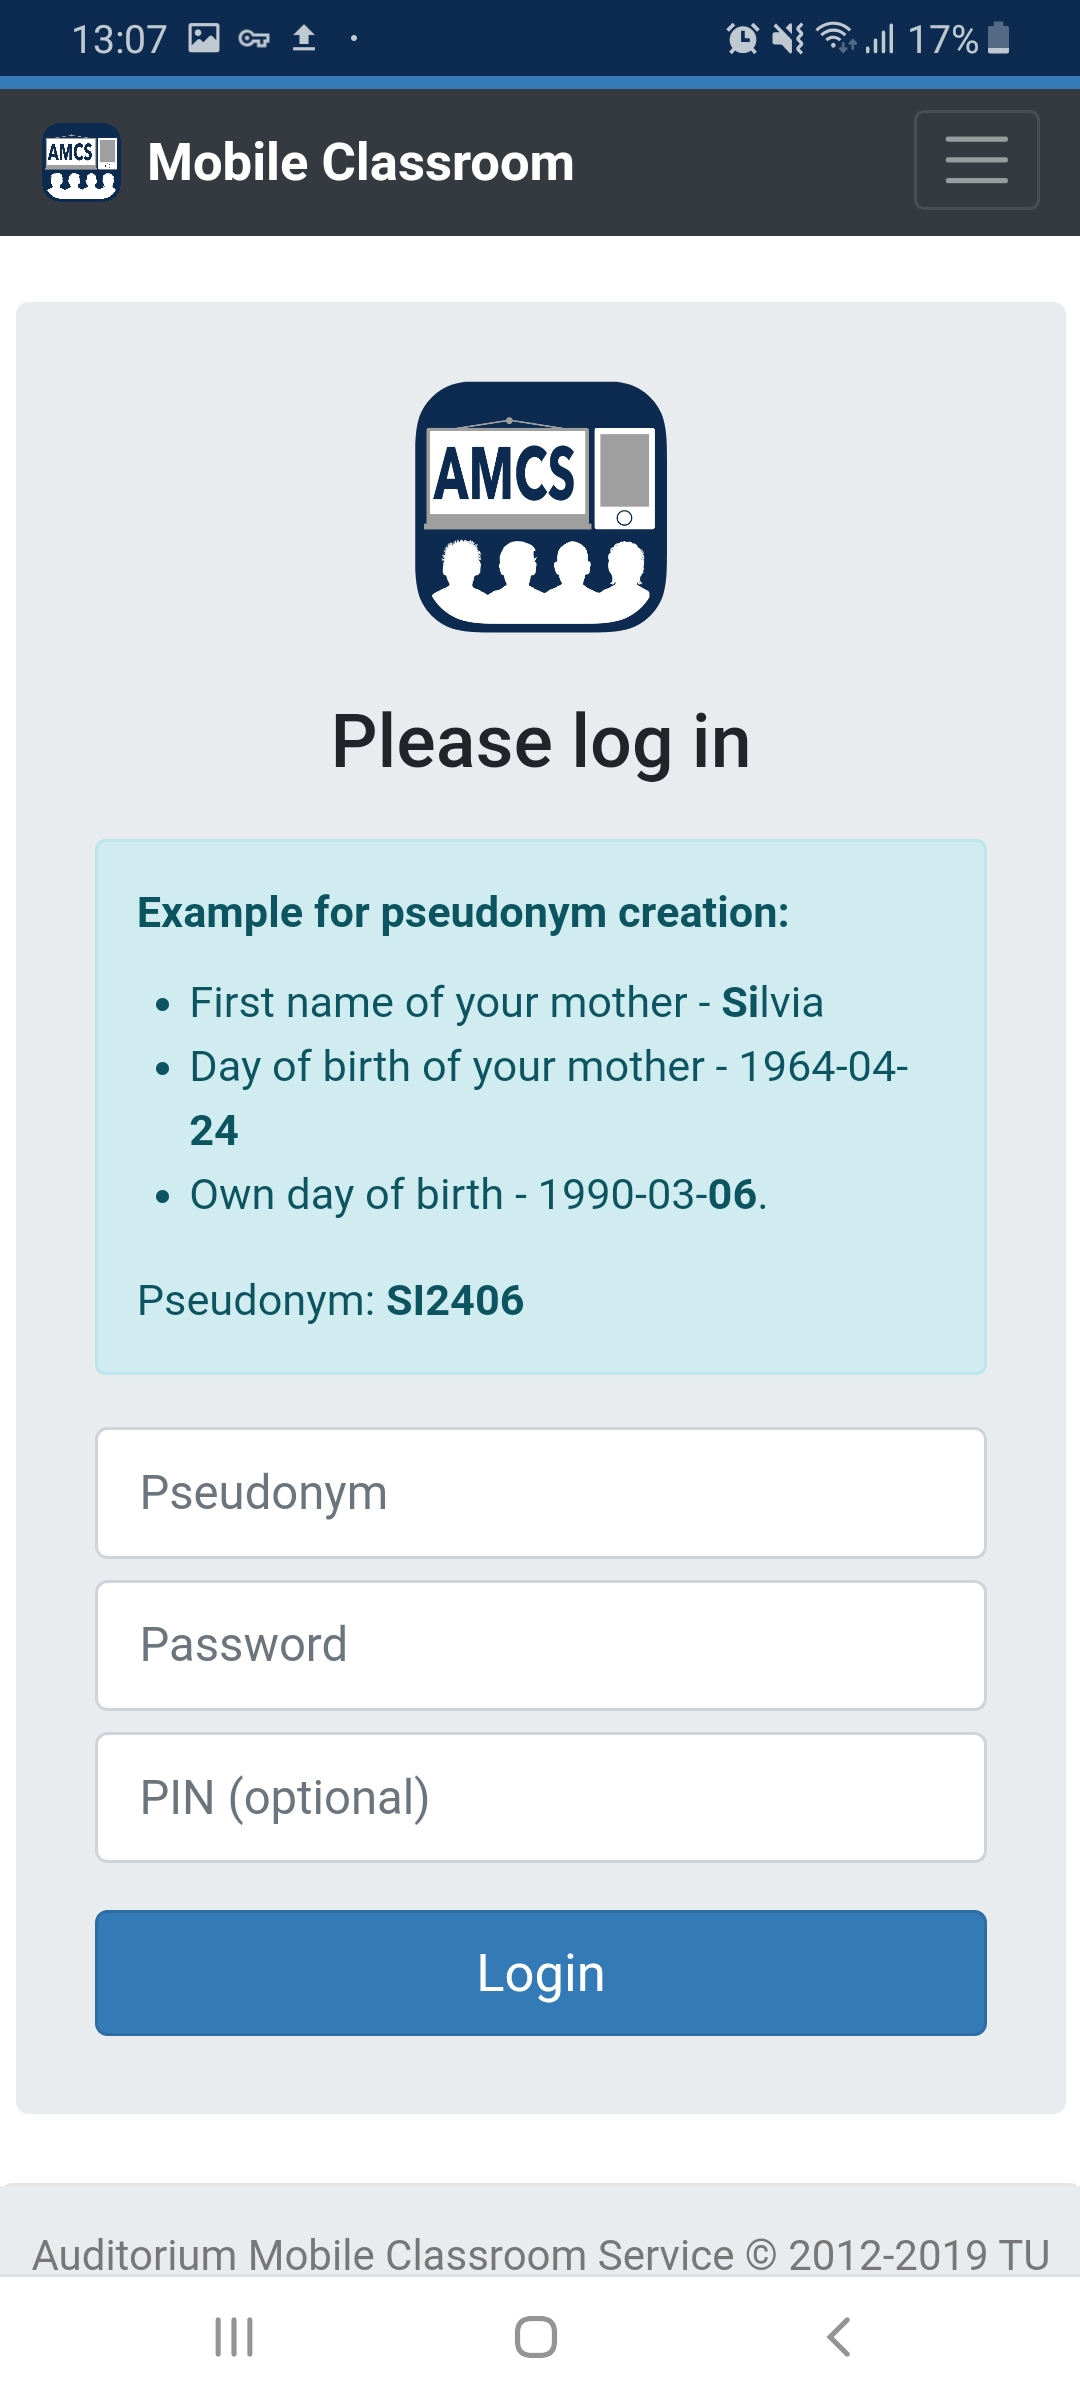
\includegraphics[width=0.95\linewidth]{screenshots/login_form.jpg}
		\captionsetup{width=.8\linewidth}
		\caption{The login form of AMCS. Users can choose a synonym and a password to create an account.}
		\label{fig:loginform}
	\end{minipage}
\end{figure}
 
\section{Main View}
\label{section:soa:mainview}
After successfully logging in, the user is presented with the Main View of the system (see \Cref{fig:mainview}).
It can be scrolled in the vertical direction and is divided into header and body. On top, the header consists of corporate branding on the left side and a burger menu on the right side. Below it, the view's body organizes information in different sections as follows:

\begin{figure}
	\centering
	\begin{minipage}[t]{.5\textwidth}
		\centering
		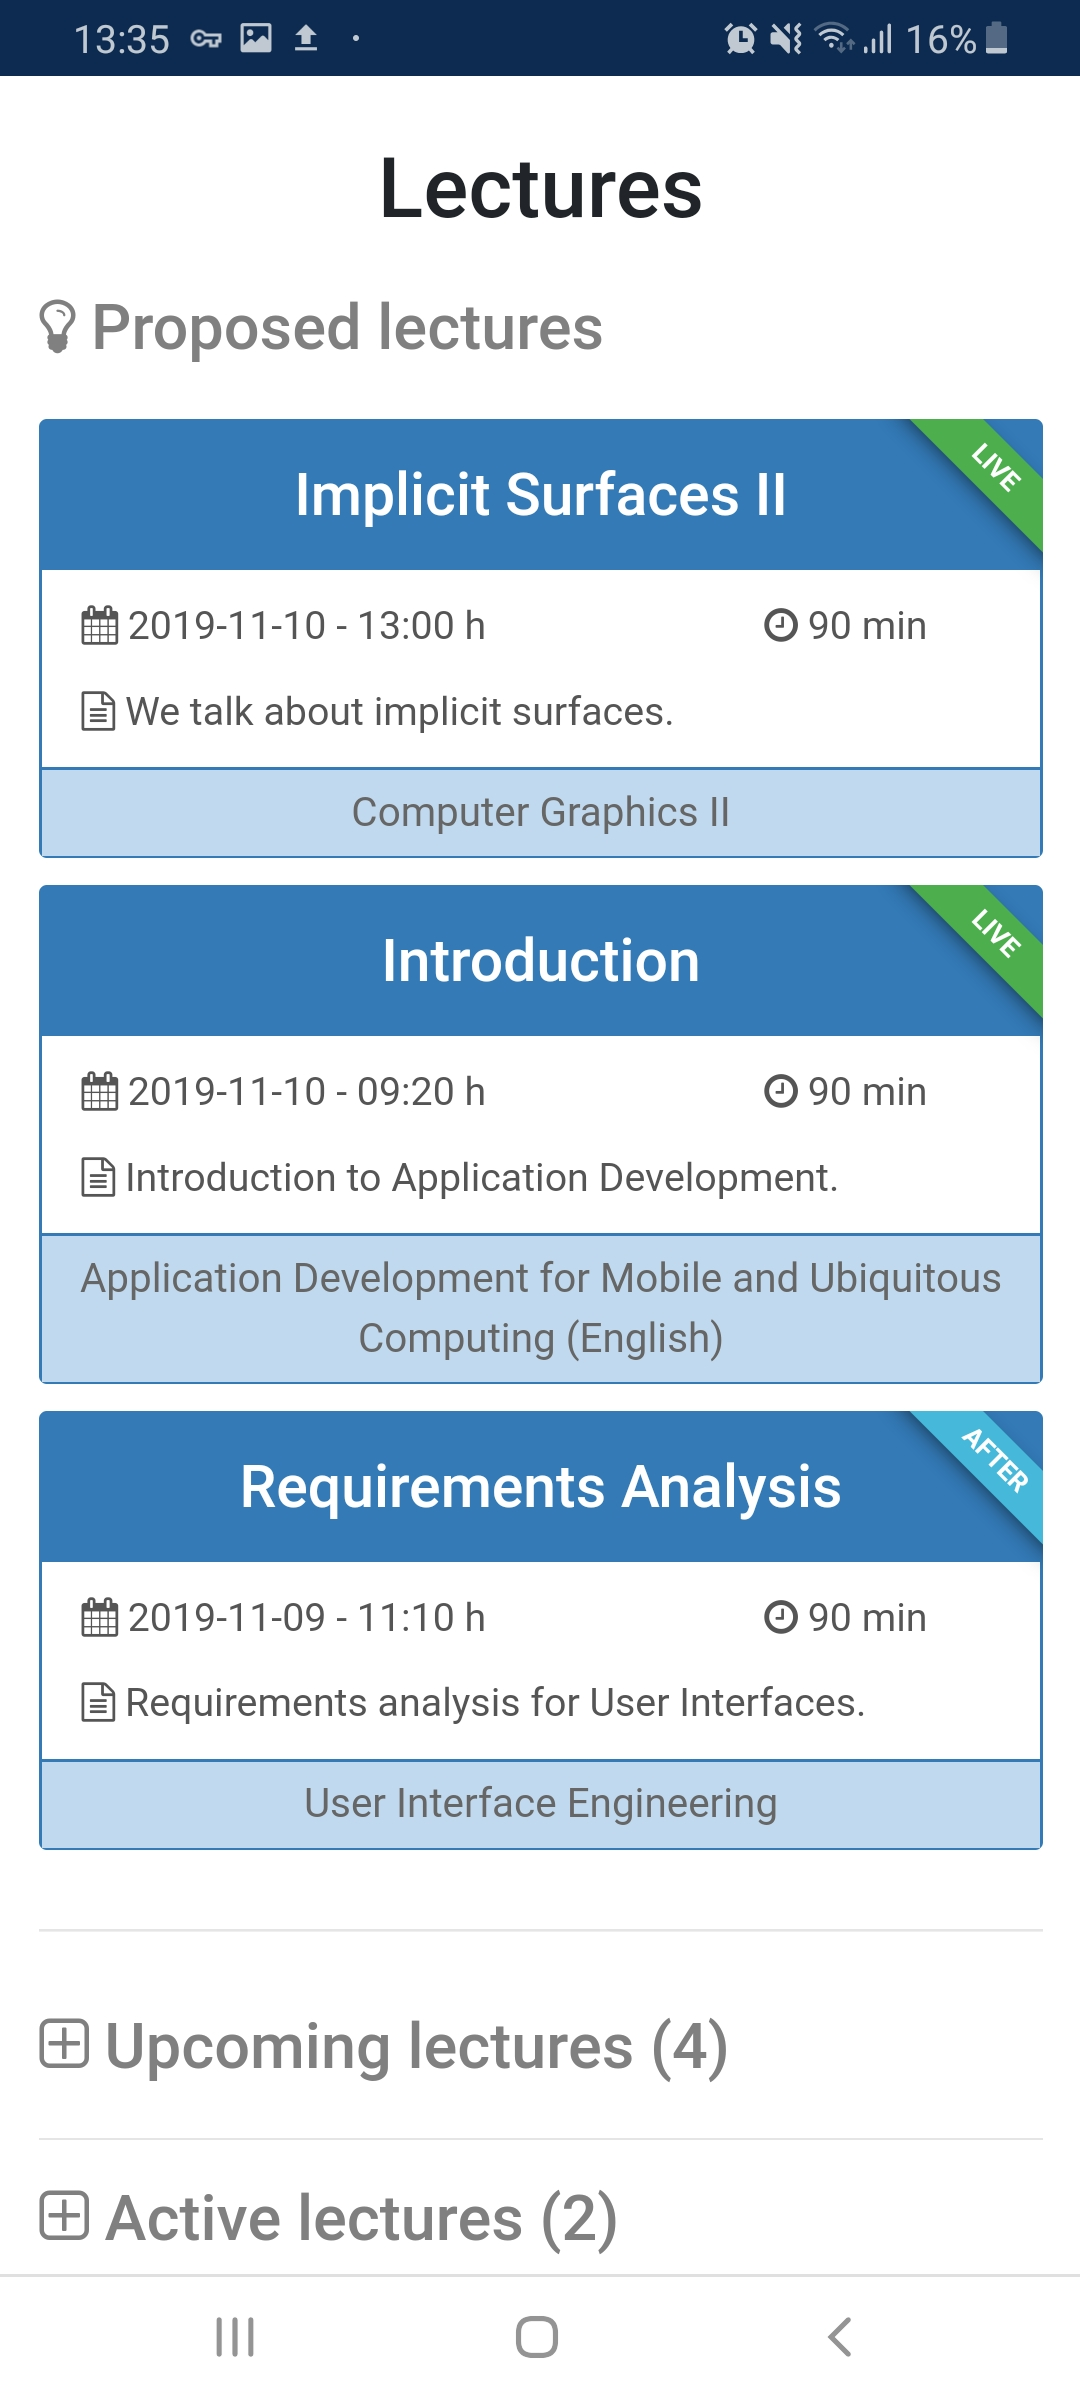
\includegraphics[width=0.95\linewidth]{screenshots/main_view_1.jpg}
		\captionsetup{width=.8\linewidth}
		\caption{Main View: Lecture information is provided in different sections for each temporal context. Per default, a section with proposed lectures is expanded.}
		\label{fig:mainview}
	\end{minipage}%
	\begin{minipage}[t]{.5\textwidth}
		\centering
		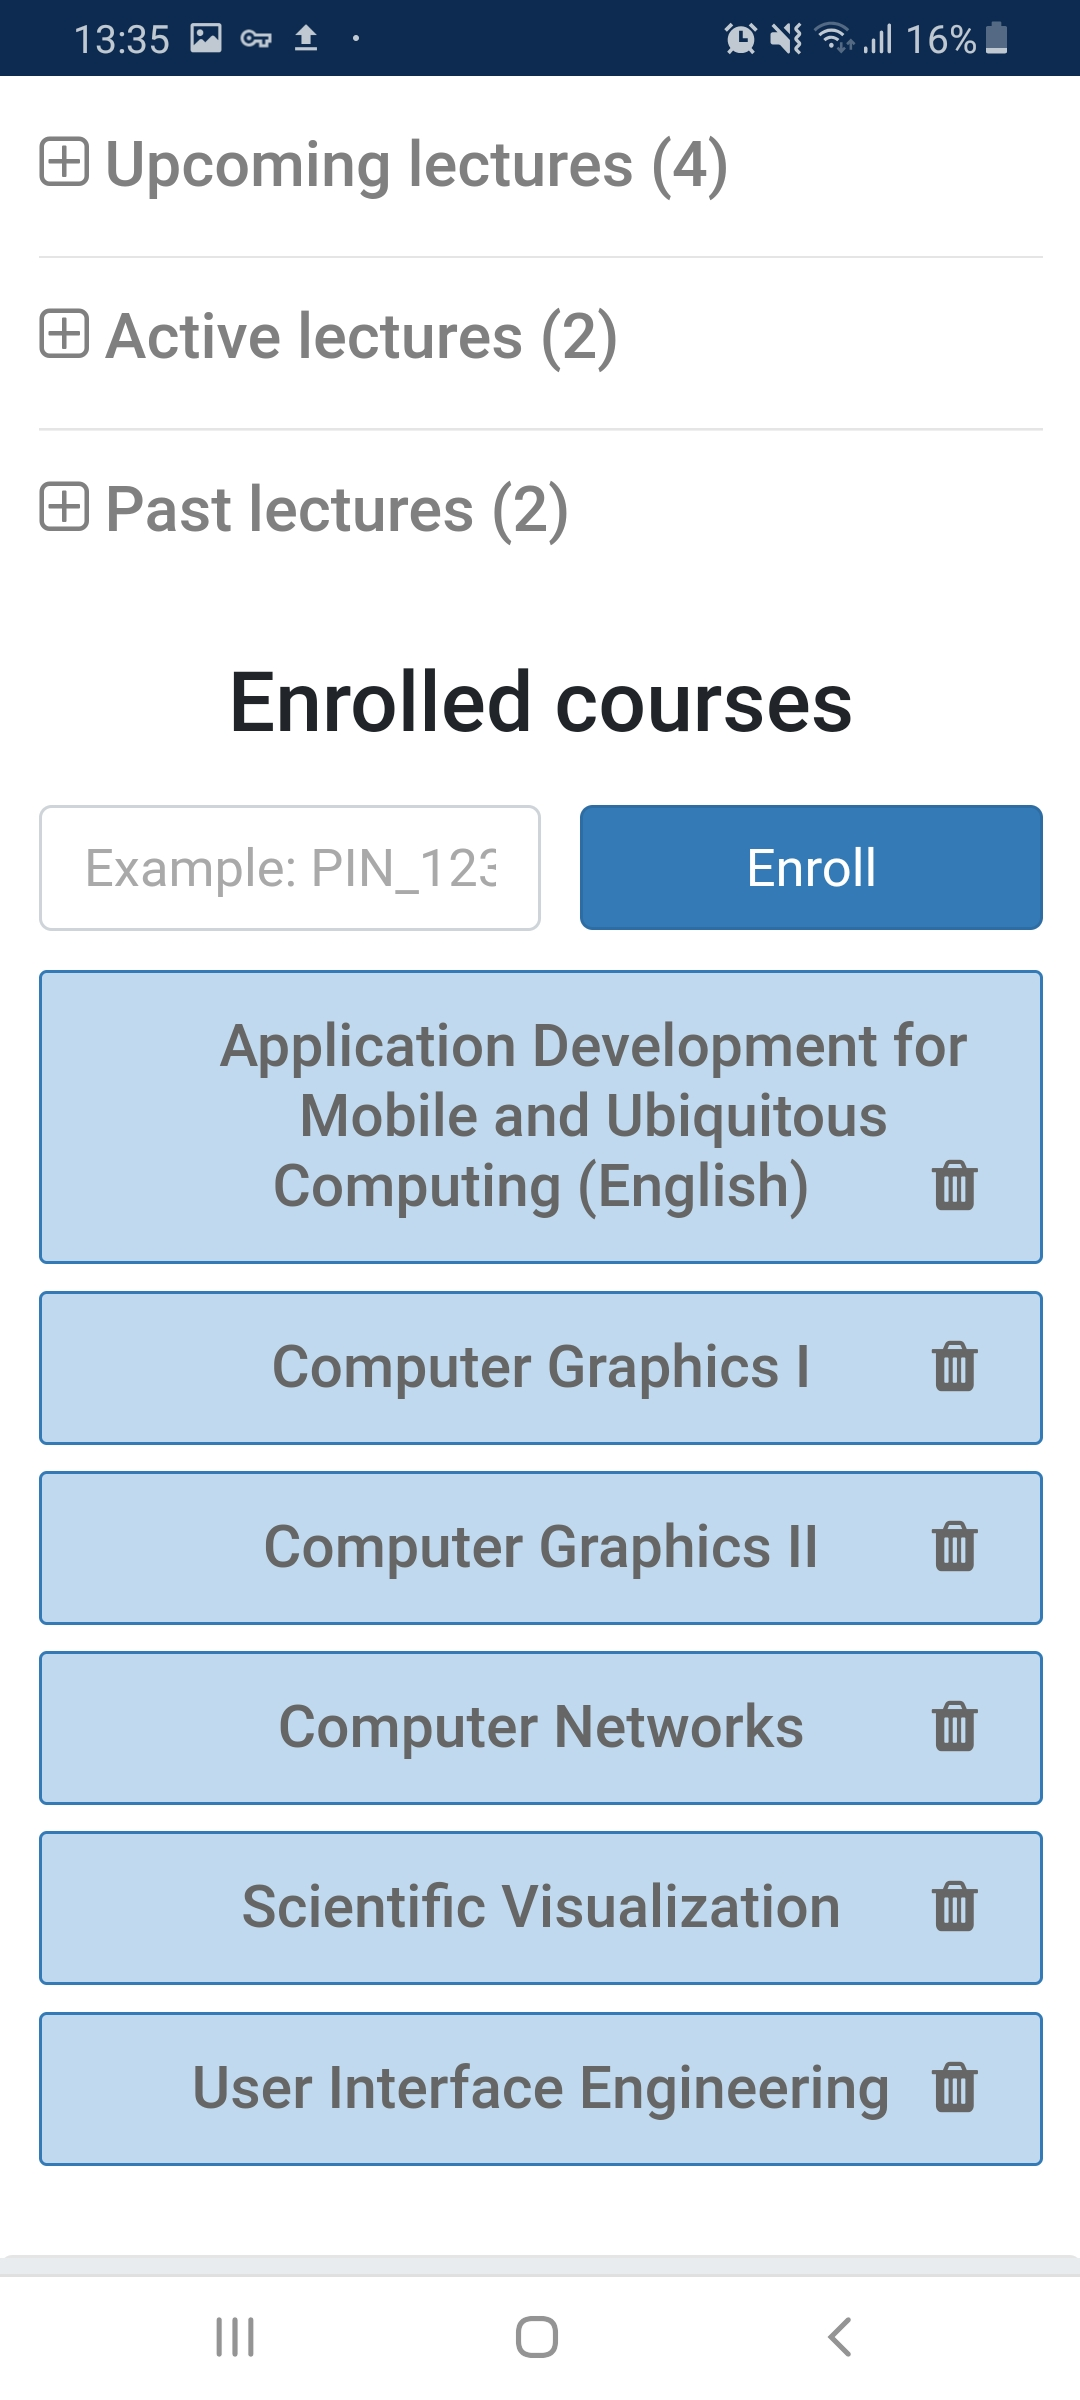
\includegraphics[width=0.95\linewidth]{screenshots/main_view_course_management.jpg}
		\captionsetup{width=.8\linewidth}
		\caption{Course management below Lectures: Each course is listed below an enrollment form consisting of a PIN input and a submit button.}
		\label{fig:mainviewcoursemanagement}
	\end{minipage}
\end{figure}

\subsection{Lectures}
\label{section:soa:mainview:lectures}
This section lists all lectures that the user subscribed to (see \Cref{fig:mainview}). It is organized in subsections that indicate the temporal context of each lecture. These include:

\paragraph{Proposed lectures} - Lectures that the system proposes to the user. These lectures either will take place in the next 24 hours or already occurred in the last 24 hours.
\paragraph{Upcoming lectures} - Lectures that will take place in the future are shown here.
\paragraph{Active lectures} - Lectures that take place right now are shown here.
\paragraph{Past lectures} - Lectures that have already taken place are shown here.

\paragraph{Rendering of lectures}

Each of the aforementioned subsections is organized in a list that contains all corresponding lectures. For each lecture, a box is rendered that uses all horizontal space available to it. The box consists of a blue header with the lecture's name, a white info/detail area and a light blue footer that contains the course name.
A color-coded badge on the top right of the boxes serves as an indicator for the temporal context of the lecture.
The subsections can be collapsed or expanded by clicking on the sections heading.

\todo{add graphic of badges}


\subsection{Course management}

Further down on the page, the section \emph{Enrolled Courses} can be found (see \Cref{fig:mainviewcoursemanagement}). It serves two purposes: Primarily, it provides a way to enroll into a course. An enrollment form is shown that consists of a text field to enter the course PIN and a blue button to trigger the enrollment. When provided with a valid PIN, pressing the button redirects the user to the \emph{Course View} (described in \Cref{section:soa:courseview}) on successful enrollment.
Secondly, the view shows all courses the student is currently enrolled in. They are rendered as light blue buttons in a vertical list. A trash can icon on each button provides a way to leave the given course.

\section{Poll View}
\label{section:soa:pollview}
Answering polls is one of the main functionalities of the system that users will engage with.
Polls can be reached by clicking on a lecture box from either the \emph{Main View} or the \emph{Course View}.
Each poll consists of a set of questions the user can answer. They are rendered in a view that is reused by the system depending on the situation and context. This means that the view might only be accessible under certain circumstances, for example when the lecture reaches a specific point in time, making it a slide poll (SP). SPs are shown when a specific slide is on display and can only be answered in this very moment. Other types of polls include “global” course polls (CP) that are always accessible during the semester and lecture polls (LP) which can only be answered during the life time of a lecture.
Active polls are displayed all at once in sections designated to each poll type.
The different types of polls that occur in AMCS are further summarized in \Cref{tab:pollTypes}.



\begin{table}[H]
	{\renewcommand{\arraystretch}{2}
		\begin{tabular}{ | p{5cm} | p{10cm} |}
			\hline
			Poll Type & Explanation \\ \hline \hline
			Slide Poll (SP) & Active when a specific slide is shown. Commonly used for quizzes after a difficult section in a lecture to make sure that students understood everything correctly. \\ \hline
			Preparation Poll (PP) & Active before the lecture takes place. Is commonly used to instruct students to prepare for a certain topic. \\ \hline
			Lecture Poll (LP) & Active during the lifetime of a lecture. \\ \hline
			Post Processing Poll (PPP) & Active after a lecture has taken place. Commonly used to check gained knowledge. \\ \hline
			Course Poll (CP) & Active during the whole lifetime of the course (commonly during the whole semester). \\
			\hline
		\end{tabular}
	}
	\caption{Different poll types that the user might encounter when using AMCS.}
	\label{tab:pollTypes}
\end{table}

If no polls for a given lecture are available, the user is presented with the hint shown in \todogrf.

\section{Course View}
\label{section:soa:courseview}

The \emph{Course View} is shown when the user selects one of the courses from the course management section (see \Cref{fig:courseview} and \Cref{fig:courseviewlectures}). Its purpose is essentially to provide a filtered view on the lectures of a single course.
The course name and PIN, it's description and lists of upcoming, live and past lectures are visible from top to bottom in this order. It reuses the lecture section component described in \Cref{section:soa:mainview:lectures}.

\begin{figure}
	\centering
	\begin{minipage}[t]{.5\textwidth}
		\centering
		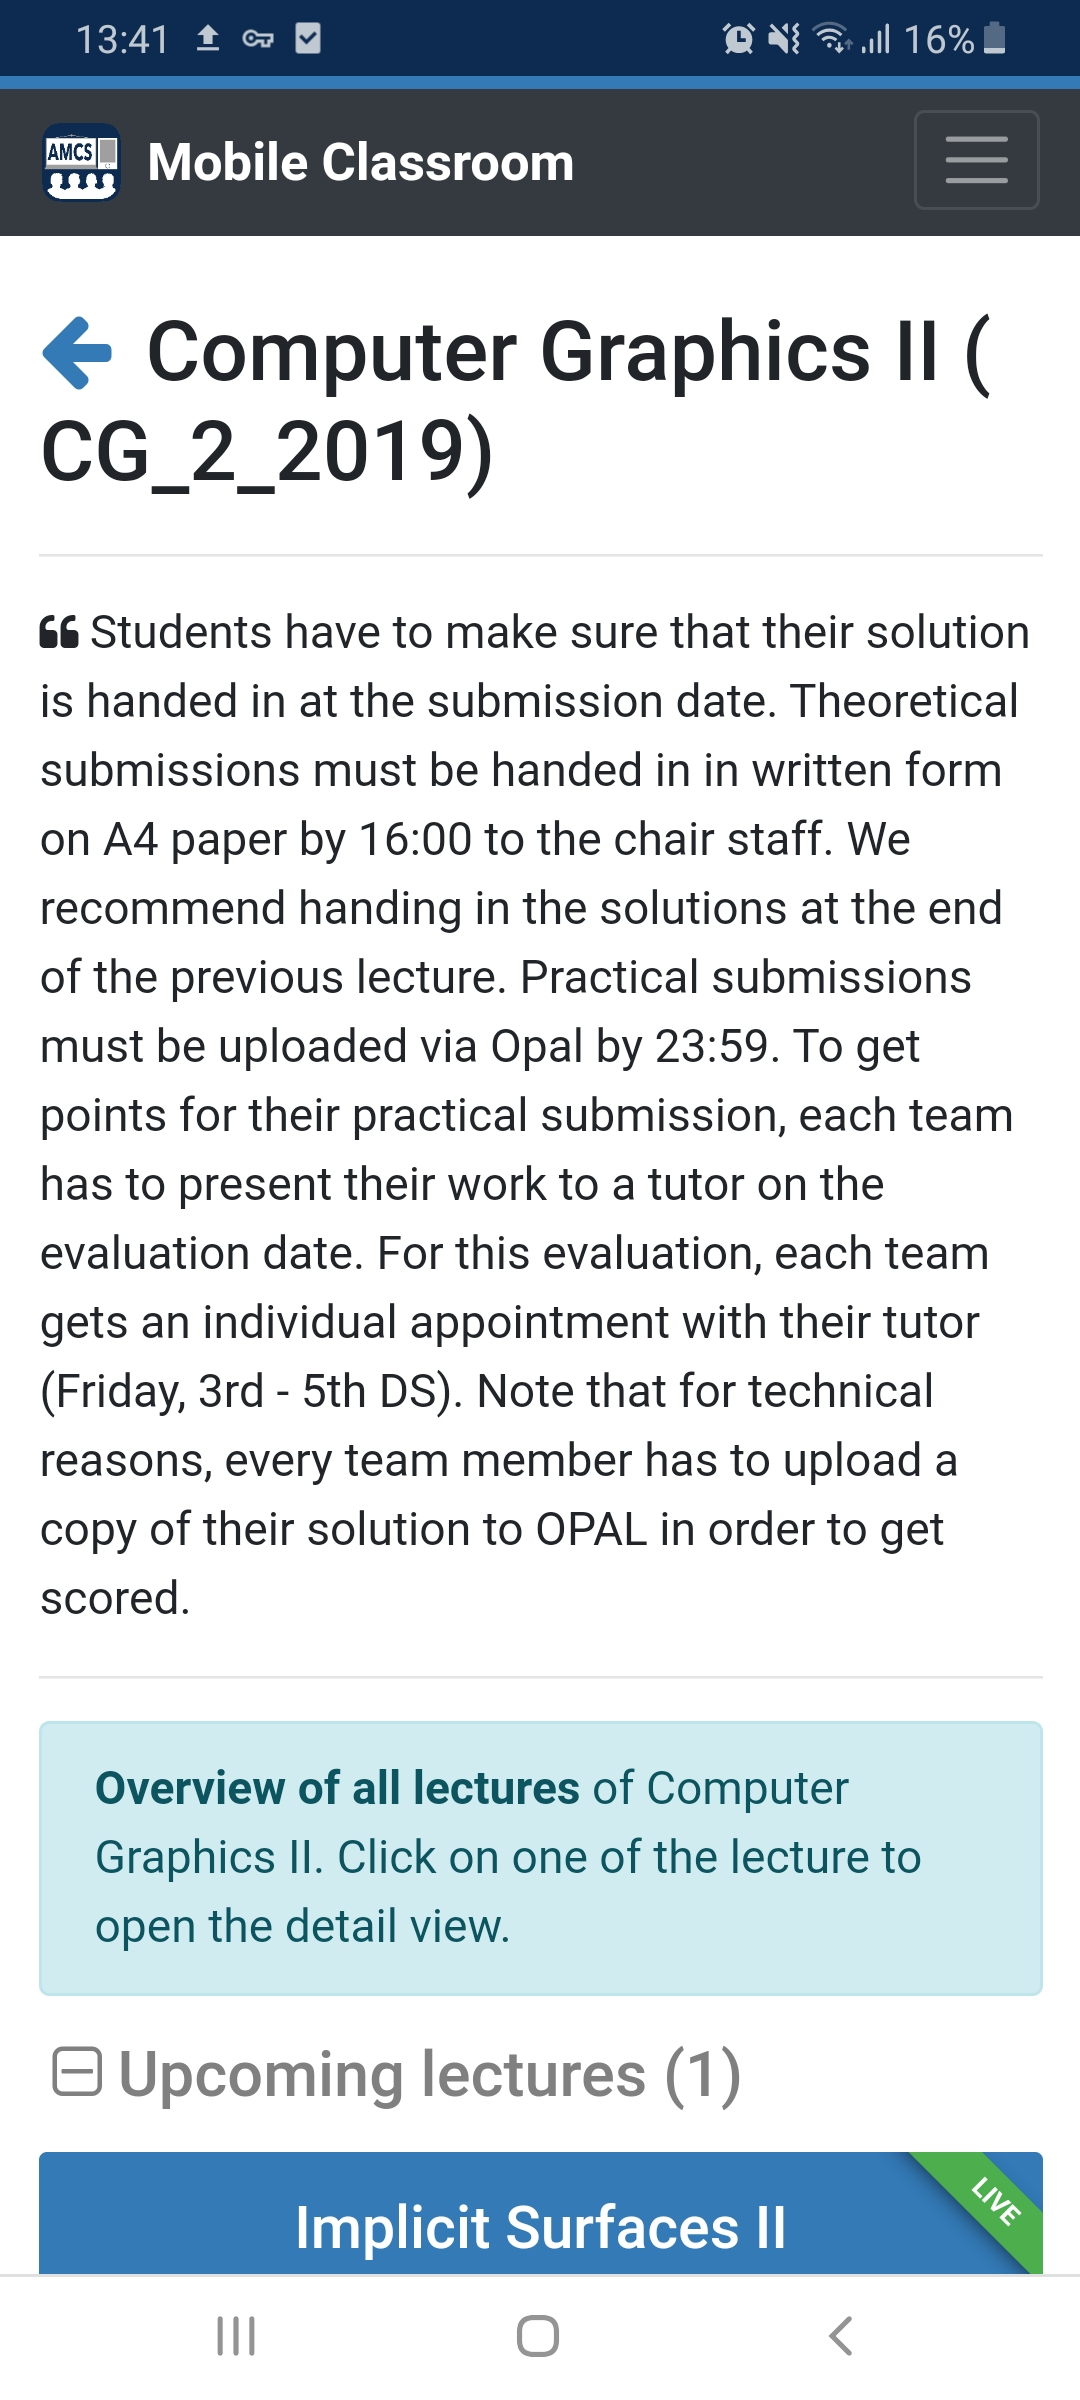
\includegraphics[width=0.95\linewidth]{screenshots/course_view_1.jpg}
		\captionsetup{width=.8\linewidth}
		\caption{\emph{Course View}: Details like the course name, description and PIN are displayed.}
		\label{fig:courseview}
	\end{minipage}%
	\begin{minipage}[t]{.5\textwidth}
		\centering
		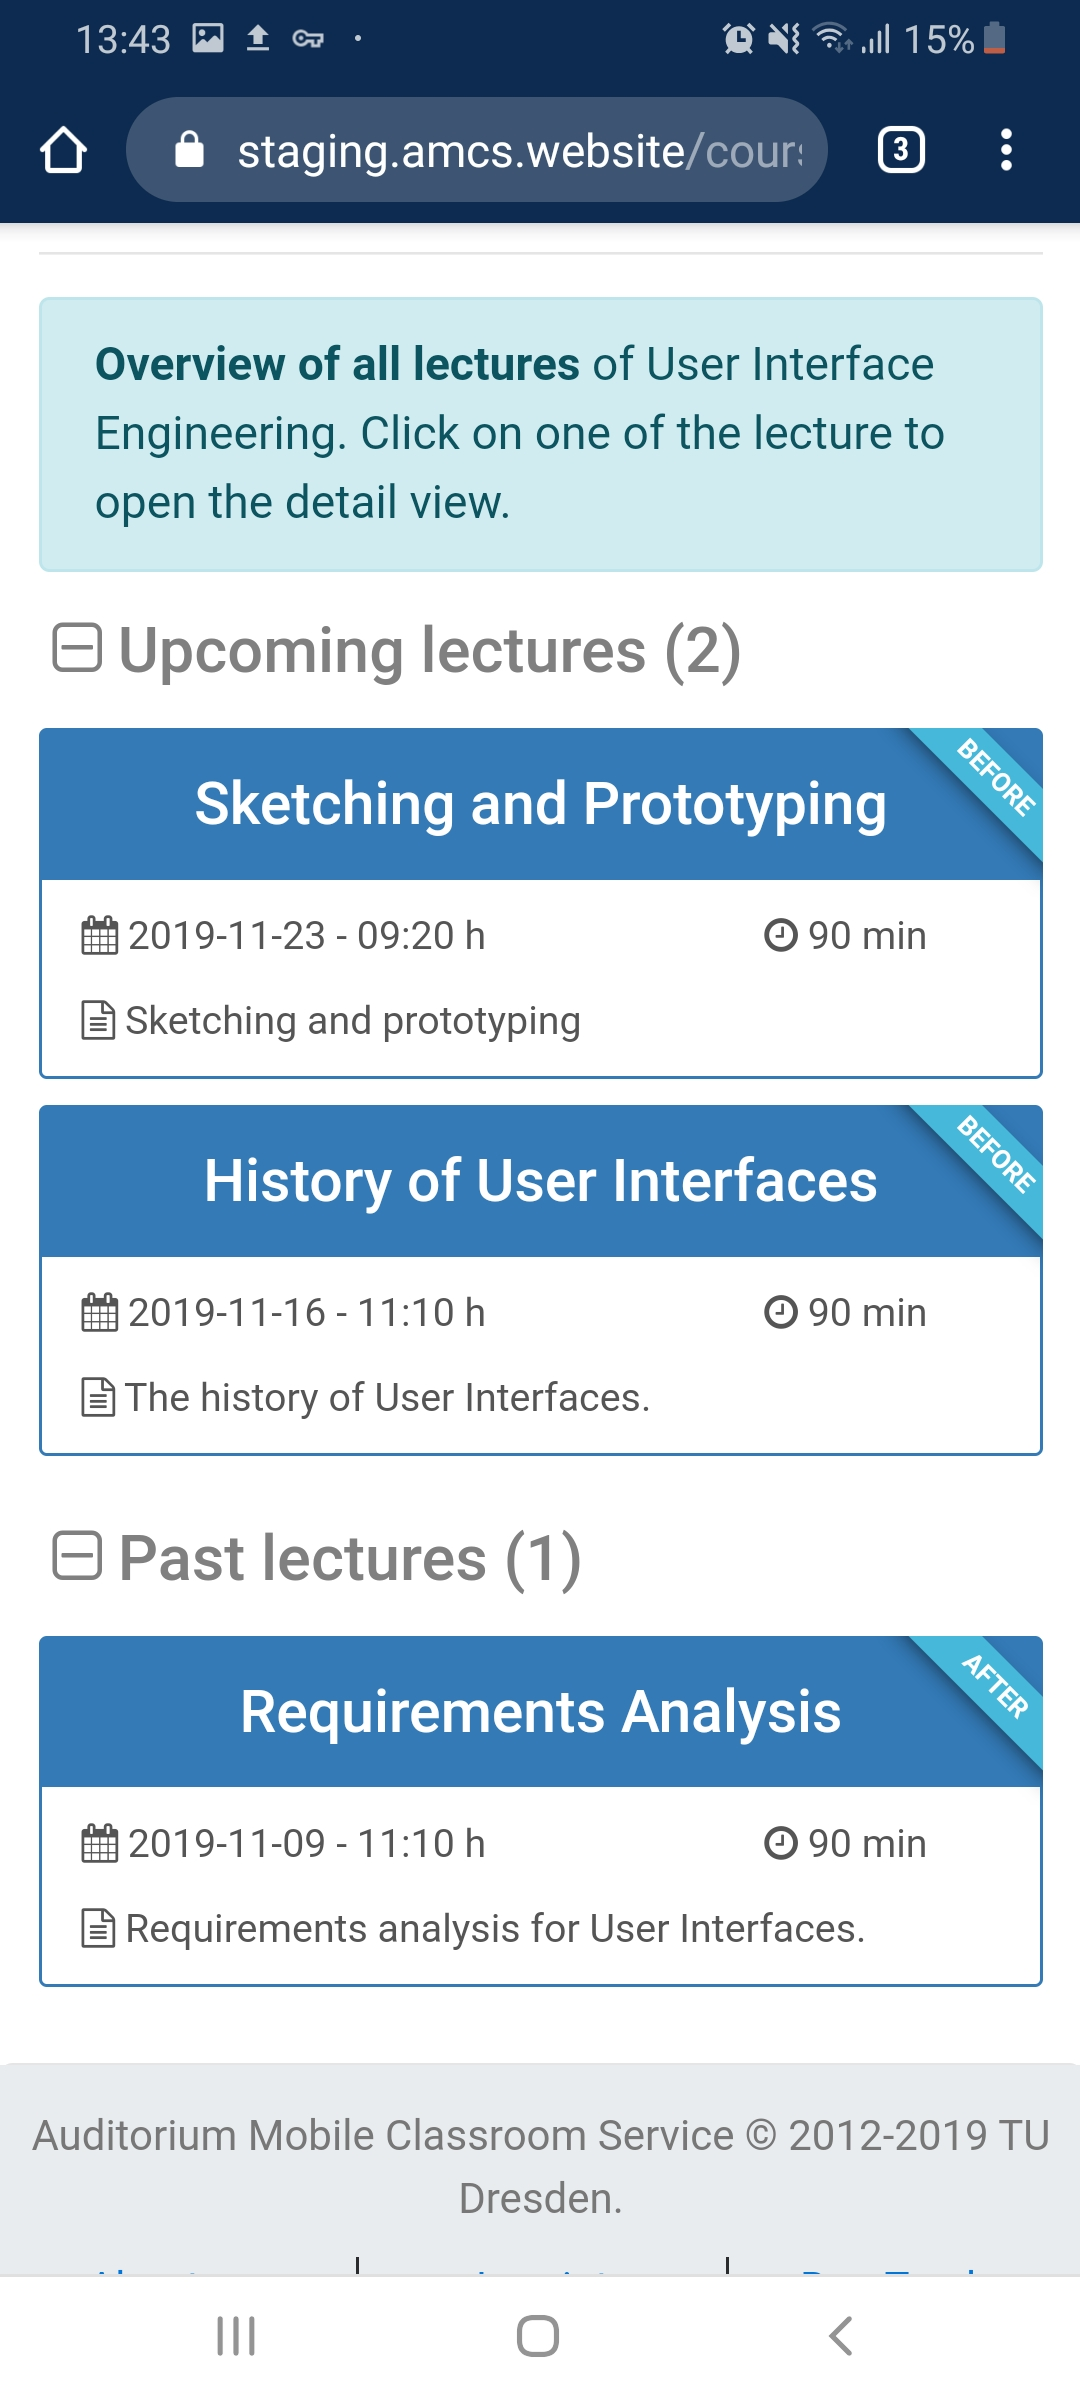
\includegraphics[width=0.95\linewidth]{screenshots/course_view_3.jpg}
		\captionsetup{width=.8\linewidth}
		\caption{Lectures that belong to a certain course displayed in the \emph{Course View}.}
		\label{fig:courseviewlectures}
	\end{minipage}
\end{figure}


\section{Menu and Navigation}
Besides using the \emph{Main View}, additional functionality can be reached by navigating the burger menu that is shown in the upper-right corner of the screen. It reveals a sub menu which expands vertically, offering three additional sub menus (see Figure \todosct). In the following, these sub menus and their functionality are briefly explained.

\subsection{Student}

This is one of the most important buttons that connects a subset of main functionalities of AMCS. Upon pressing this button, the menu expands again vertically, showing a list of further sub menus. Most of the functionalities shown in this list will be touched by the proposals for improvement that are presented in \Cref{chapter:concept}. The functionalities in questions are:

\begin{enumerate}
	\item Evaluation of answers
	\item Question Pool
	\item Edit account
\end{enumerate}

\subsubsection{Evaluation of Answers}

Once students have participated in a poll and answered a few questions, they can evaluate their answers by selecting this option. Two drop down menus are shown prompting the student to select the course and lecture they are interested in. 
After choosing an item from the list, a vertical list of all questions that occurred during this lecture is shown to the student, together with indicators for the given answers.
If the student used two attempts to answer the question, a toggle button is provided to switch between the first and the second answer. \todogrf

\subsubsection{Question Pool}

By selecting this option from the \emph{Burger Menu}, the student is offered the possibility to create collections of already answered questions. The intent is to provide a way for students to collect and repeat questions that they had difficulty in answering.
Similar to \todosct, the student is prompted with a drop down menu to select a course they are interested in. After selection, the student is presented with a list of all lectures and their polls respectively. All questions of each poll are grouped and shown to the student in a vertical list. From this list, the student can select all questions that they might be interested in to create a pool of questions.
These pools are composed into polls that the student then can answer again. These polls are rendered in the same manner as stated in \Cref{section:soa:pollview}.


\subsubsection{How It Works}

Pressing this button will redirect to a page that shows tutorial instructions on how to use AMCS.
This help page is rendered identical on all mobile devices and therefore falls out of the scope of this paper.

\subsubsection{Logout}

As the name already states, pressing this button will logout the user and end the session. 
If logging out was successful, the \emph{Landing Page} is displayed.




\begin{figure}
	\centering
	\begin{minipage}[t]{.5\textwidth}
		\centering
		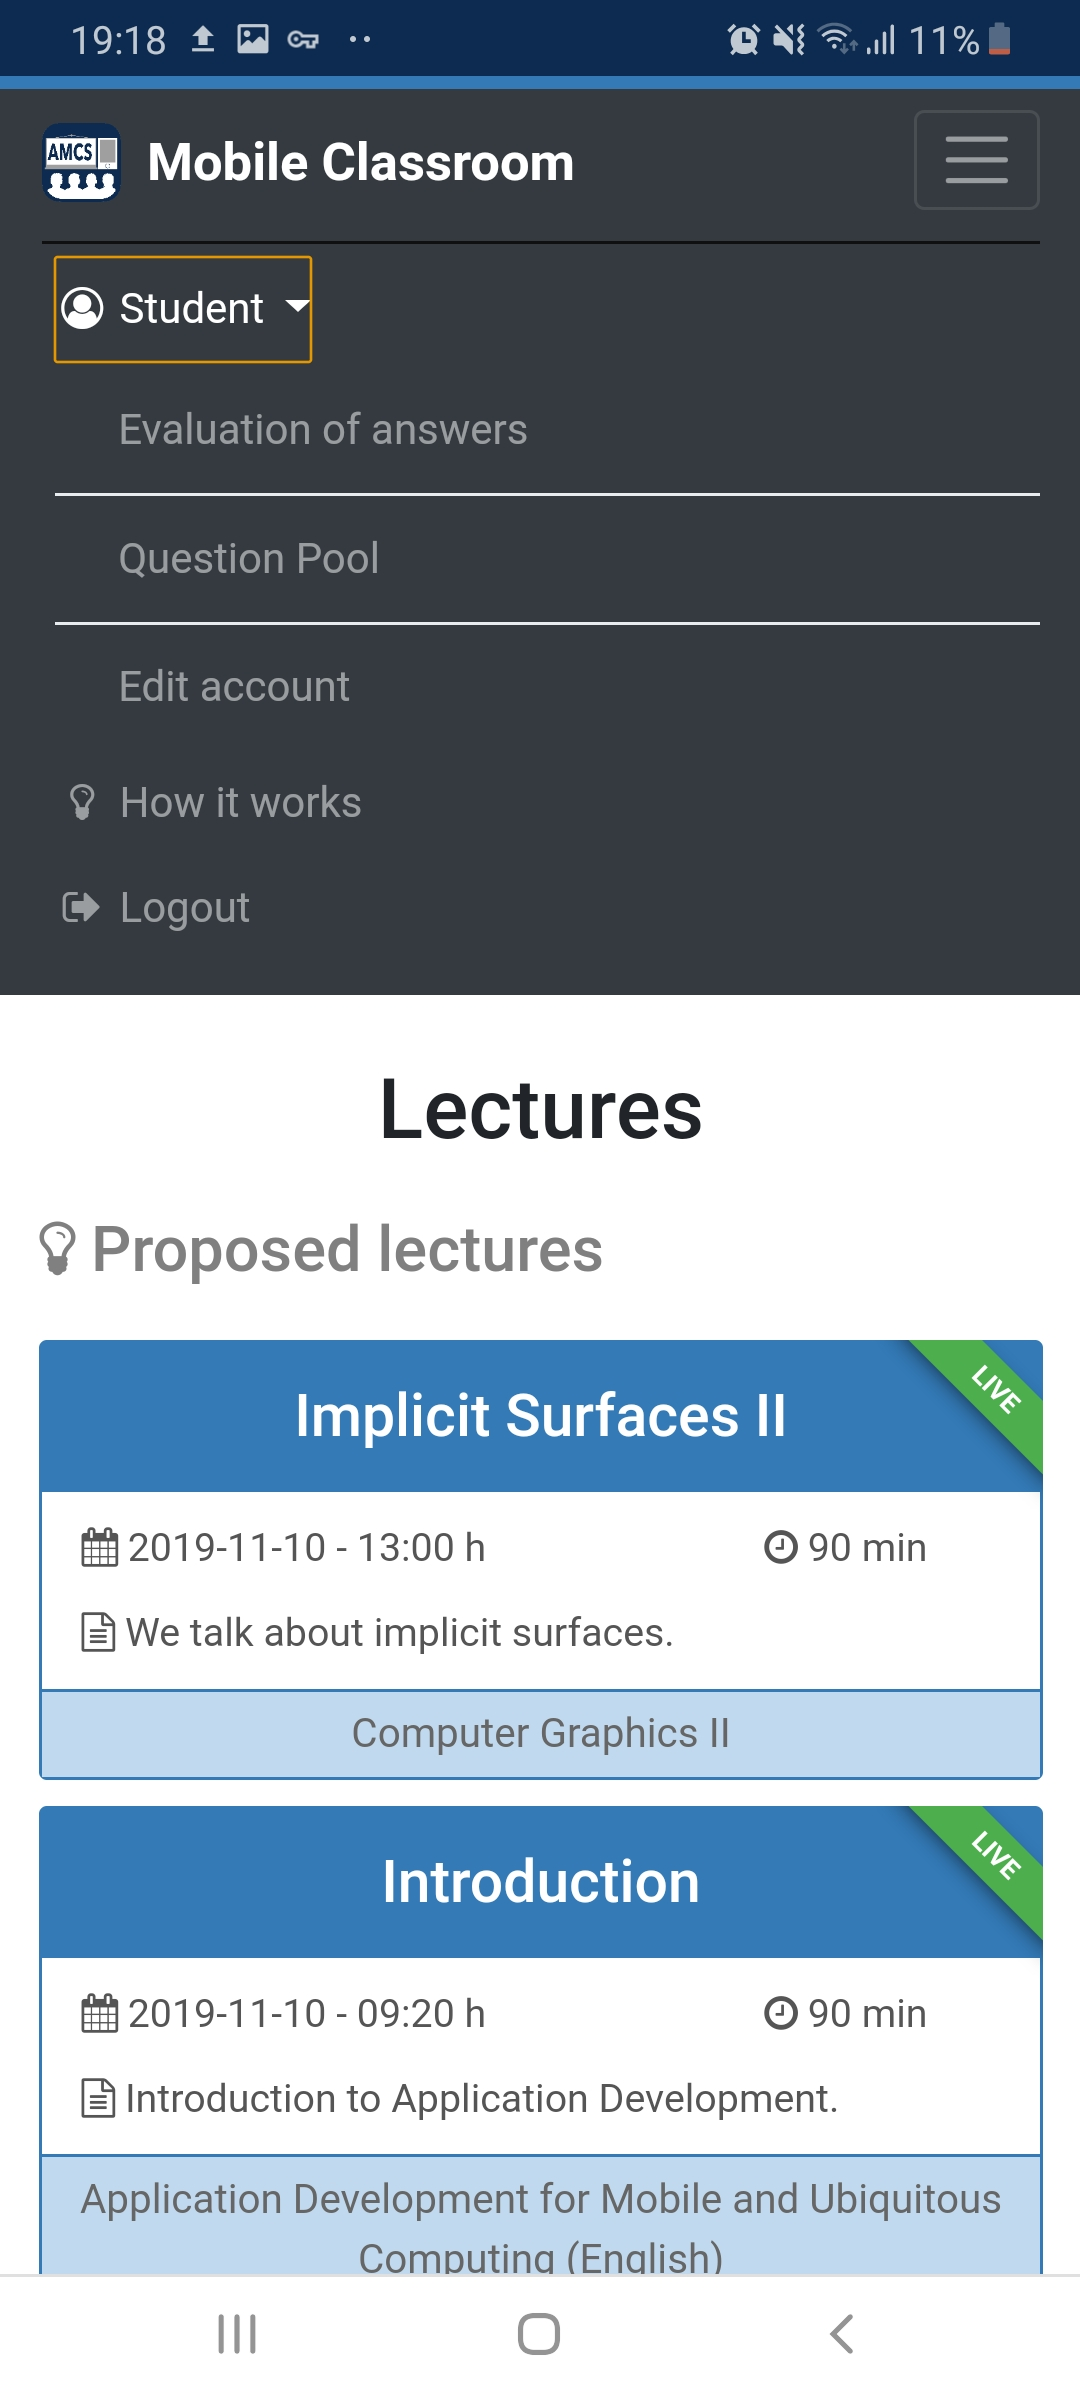
\includegraphics[width=0.95\linewidth]{screenshots/expanded_burger_menu.jpg}
		\captionsetup{width=.8\linewidth}
		\caption{Expanded \emph{Burger Menu}.}
		\label{fig:menu}
	\end{minipage}%
	\begin{minipage}[t]{.5\textwidth}
		\centering
		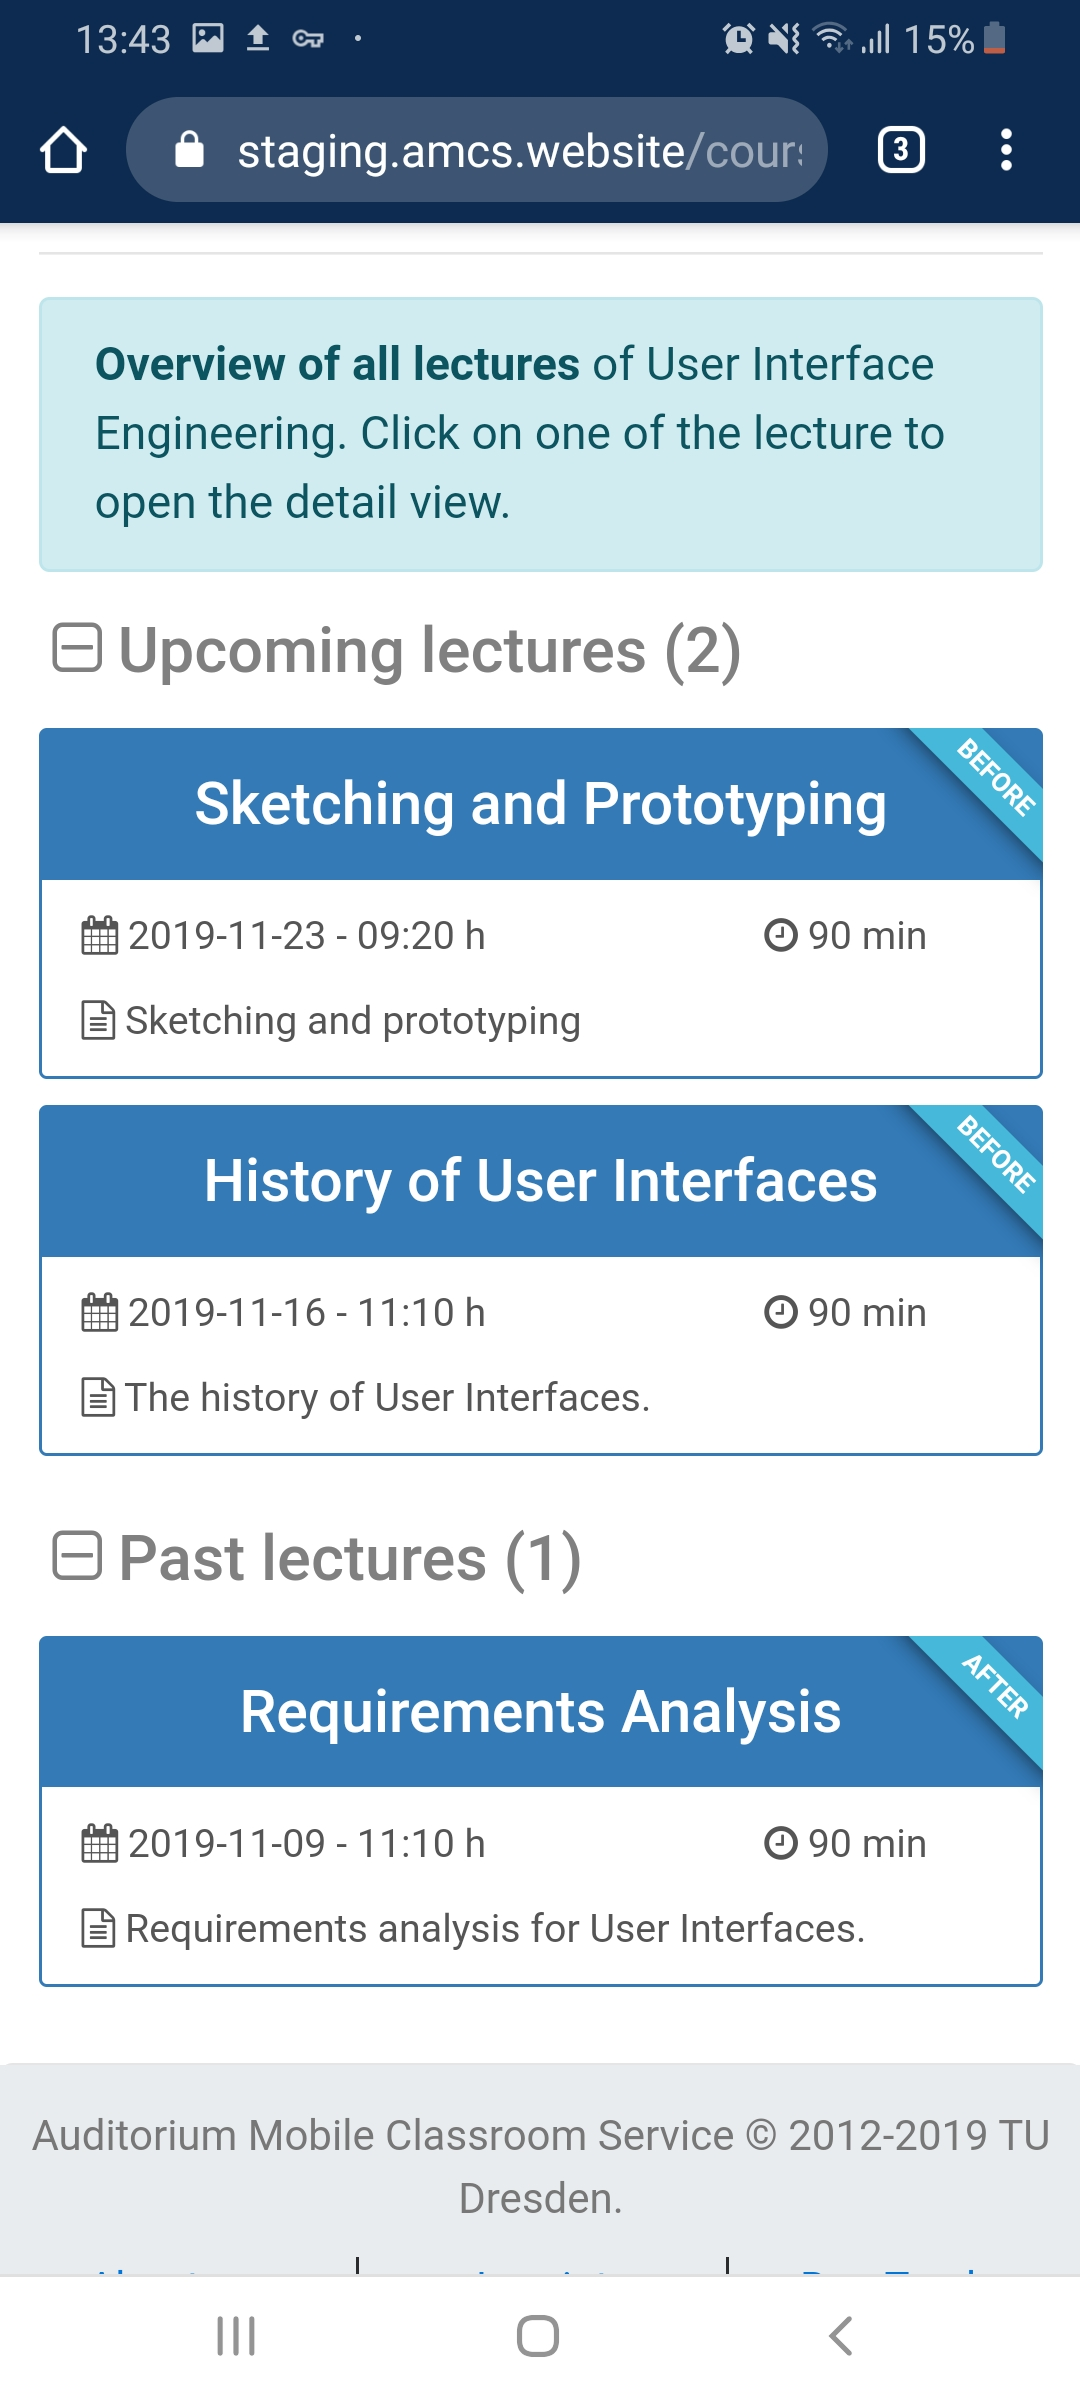
\includegraphics[width=0.95\linewidth]{screenshots/course_view_3.jpg}
		\captionsetup{width=.8\linewidth}
		\caption{Lectures that belong to a certain course displayed in the \emph{Course View}.}
		\label{fig:other}
	\end{minipage}
\end{figure}

\section{Summary}
The identified UI components that will be further analyzed and discussed are summarized in the following table:

\begin{table}[H]
	{\renewcommand{\arraystretch}{2}
		\begin{tabular}{ | p{4cm} | p{11cm} |}
			\hline
			Component & Description \\ \hline \hline
			Landing Page & Shown when the web page is opened. Points to the Login mechanism. \\ \hline
			Main View & Gives an overview of ongoing lectures and enrolled courses. Allows to enroll to or unsubscribe from courses. \\ \hline
			Poll View & Shown whenever a poll should be answered. \\ \hline
			Course View & Displays information and lectures of a single course. \\ \hline
			Burger Menu & Overarching navigation element visible in all views. \\ \hline
			Question Pool & Shown when the creation of a question pool is attempted. Can be reached from the \emph{Burger Menu}. \\ \hline
			Evaluation of answers & Shown when the evaluation of answers to polls is attempted. Can be reached from the \emph{Burger Menu}. \\ \hline
		\end{tabular}
	}
	\caption{Summary of UI Components discussed in this work.}
	\label{tab:components}
\end{table}

